\documentclass[12pt,a4paper]{article}
\usepackage[utf8]{inputenc}
\usepackage{tikz}
\usetikzlibrary{shapes,arrows,positioning,decorations.pathreplacing,calc,fit,backgrounds}
\usepackage{geometry}
\usepackage{setspace}
\usepackage{hyperref}
\geometry{margin=1in}

\title{Lightweight Threat Modeler: A Browser-Native Hybrid Pipeline for STRIDE and DREAD Security Analysis}
\author{System Research Documentation}
\date{\today}

\begin{document}
\maketitle
\onehalfspacing

\begin{abstract}
This article documents the architecture and analytical workflow of the Lightweight Threat Modeler, a browser-native security engineering tool for structured threat modeling. The system combines deterministic repository extraction, typed component intelligence, and LLM-assisted reasoning to produce reproducible STRIDE threat catalogs and DREAD prioritization outputs. Unlike purely prompt-driven systems, the tool grounds model reasoning in build-system manifests, file structure, import-graph signals, and curated domain security templates. The resulting pipeline supports both greenfield and brownfield applications, with explicit trust-boundary modeling, questionnaire-guided elicitation, and machine-readable report export for downstream governance.
\end{abstract}

\section{Introduction}
Threat modeling quality often degrades when model outputs are not anchored to implementation evidence. Lightweight Threat Modeler addresses this by combining:
\begin{itemize}
    \item deterministic extraction from project ZIP archives,
    \item curated component taxonomy with pre-mapped STRIDE threats,
    \item guided human-in-the-loop questionnaire triage,
    \item selective Gemini-assisted augmentation for analysis and remediation.
\end{itemize}

The design emphasizes practical security workflows: rapid model bootstrap, transparent threat provenance, and export-ready artifacts for engineering and compliance programs.

\section{System Architecture Overview}
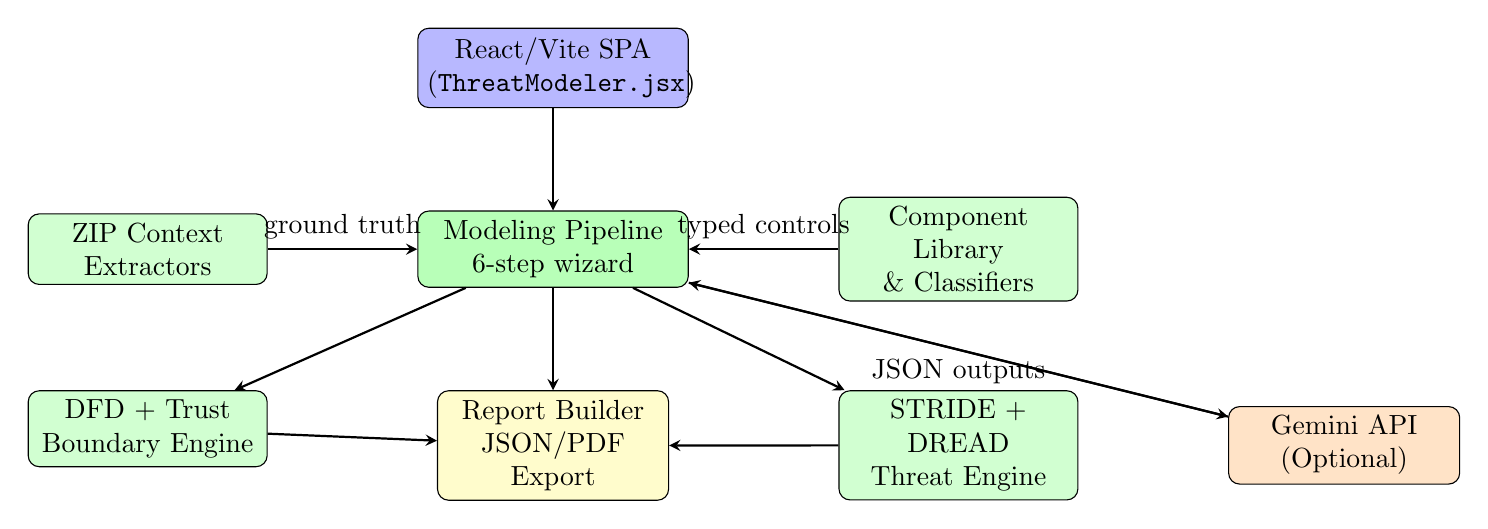
\begin{tikzpicture}[
    node distance=1.3cm and 1.9cm,
    box/.style={rectangle, draw, rounded corners, text width=3.2cm, text centered, minimum height=0.95cm, fill=blue!18},
    proc/.style={rectangle, draw, rounded corners, text width=2.8cm, text centered, minimum height=0.85cm, fill=green!18},
    data/.style={rectangle, draw, rounded corners, text width=2.7cm, text centered, minimum height=0.8cm, fill=yellow!20},
    ext/.style={rectangle, draw, rounded corners, text width=2.7cm, text centered, minimum height=0.85cm, fill=orange!22},
    arrow/.style={->, >=stealth, thick}
]
    \node[box, fill=blue!28] (ui) {React/Vite SPA\\(\texttt{ThreatModeler.jsx})};
    \node[box, below=of ui, fill=green!28] (pipeline) {Modeling Pipeline\\6-step wizard};
    \node[proc, left=of pipeline] (zip) {ZIP Context\\Extractors};
    \node[proc, right=of pipeline] (library) {Component Library\\\& Classifiers};
    \node[proc, below left=of pipeline] (dfd) {DFD + Trust\\Boundary Engine};
    \node[proc, below right=of pipeline] (stride) {STRIDE + DREAD\\Threat Engine};
    \node[data, below=of pipeline] (report) {Report Builder\\JSON/PDF Export};
    \node[ext, right=of stride] (gemini) {Gemini API\\(Optional)};

    \draw[arrow] (ui) -- (pipeline);
    \draw[arrow] (zip) -- node[above] {ground truth} (pipeline);
    \draw[arrow] (library) -- node[above] {typed controls} (pipeline);
    \draw[arrow] (pipeline) -- (dfd);
    \draw[arrow] (pipeline) -- (stride);
    \draw[arrow] (dfd) -- (report);
    \draw[arrow] (stride) -- (report);
    \draw[arrow] (pipeline) -- (report);
    \draw[arrow] (pipeline) -- (gemini);
    \draw[arrow] (gemini) -- node[below] {JSON outputs} (pipeline);
\end{tikzpicture}

\newpage
\section{Wizard-Centric Operational Flow}
\begin{tikzpicture}[
    node distance=0.95cm and 1.5cm,
    step/.style={rectangle, draw, rounded corners, text width=3.3cm, text centered, minimum height=0.85cm, fill=blue!15},
    aux/.style={rectangle, draw, rounded corners, text width=3cm, text centered, minimum height=0.75cm, fill=green!15},
    arrow/.style={->, >=stealth, thick}
]
    \node[step, fill=blue!25] (s1) {Step 1\\Application Profile\\(+ optional ZIP/context)};
    \node[step, below=of s1] (s2) {Step 2\\Module Decomposition\\(deterministic + AI)};
    \node[step, below=of s2] (s3) {Step 3\\DFD \& Trust Boundaries};
    \node[step, below=of s3] (s4) {Step 4\\STRIDE Threat Analysis};
    \node[step, below=of s4] (s5) {Step 5\\DREAD Risk Scoring};
    \node[step, below=of s5, fill=blue!25] (s6) {Step 6\\Threat Modeling Report};

    \node[aux, right=2.0cm of s2] (cls) {Rule/AI\\Component Classification};
    \node[aux, right=2.0cm of s4] (q) {Questionnaire +\\Library Seeding};
    \node[aux, right=2.0cm of s6] (exp) {Export\\JSON / Print PDF};

    \draw[arrow] (s1) -- (s2);
    \draw[arrow] (s2) -- (s3);
    \draw[arrow] (s3) -- (s4);
    \draw[arrow] (s4) -- (s5);
    \draw[arrow] (s5) -- (s6);

    \draw[arrow] (s2) -- (cls);
    \draw[arrow] (cls) -- (s2);
    \draw[arrow] (s4) -- (q);
    \draw[arrow] (q) -- (s4);
    \draw[arrow] (s6) -- (exp);
\end{tikzpicture}

\section{Deterministic Grounding from Project ZIP}
The pipeline intentionally runs deterministic extraction before any LLM call:
\begin{itemize}
    \item \textbf{Structural extractor} (\texttt{projectStructureModules.js}): parses manifests and layout (\texttt{package.json} workspaces, \texttt{pnpm-workspace.yaml}, \texttt{lerna.json}, \texttt{pom.xml}, \texttt{go.work}, top-level folders).
    \item \textbf{Import extractor} (\texttt{codeImportModules.js}): parses JS/TS import specifiers and clusters code by directory affinity and external dependency signatures.
    \item \textbf{Context extractor} (\texttt{projectZipContext.js}): creates bounded text context (file index + key manifests/readmes) for grounded prompting.
\end{itemize}

\begin{tikzpicture}[
    x=1cm, y=1cm,
    proc/.style={rectangle, draw, rounded corners, text width=3.1cm, text centered, minimum height=0.95cm, fill=green!20},
    data/.style={rectangle, draw, rounded corners, text width=3.0cm, text centered, minimum height=0.9cm, fill=yellow!22},
    out/.style={rectangle, draw, rounded corners, text width=5.9cm, text centered, minimum height=0.9cm, fill=blue!20},
    arrow/.style={->, >=stealth, thick}
]
    \node[data] (zip) at (0,0) {Input ZIP Archive\\(client-side only)};

    \node[proc] (struct) at (-5.4,-2.8) {Structural Signal\\Extractor};
    \node[proc] (imports) at (0,-2.8) {Import Graph\\Extractor};
    \node[proc] (ctx) at (5.4,-2.8) {Manifest/README\\Context Extractor};

    \node[out] (signals) at (0,-5.6) {Deterministic Signal Bundle\\(module names, dependencies, inter-module flows)};
    \node[out, fill=blue!28] (fallback) at (0,-7.9) {Fallback Module Set\\(no-LLM-safe mode)};

    \draw[arrow] (zip) -- (struct);
    \draw[arrow] (zip) -- (imports);
    \draw[arrow] (zip) -- (ctx);
    \draw[arrow] (struct) -- (signals);
    \draw[arrow] (imports) -- (signals);
    \draw[arrow] (ctx) -- (signals);
    \draw[arrow] (signals) -- (fallback);
\end{tikzpicture}

\newpage
\section{Hybrid Module Typing and Threat Seeding}
Modules are typed against a curated taxonomy in \texttt{componentLibrary.json}. Each type contains:
\begin{itemize}
    \item detection hints (\texttt{depNames}, \texttt{fileRegex}, \texttt{envKeys}, \texttt{nameKeywords}),
    \item default architecture fields (inputs/outputs/stores/entities),
    \item predefined STRIDE threat templates,
    \item mapped security requirements (e.g., OWASP ASVS families).
\end{itemize}

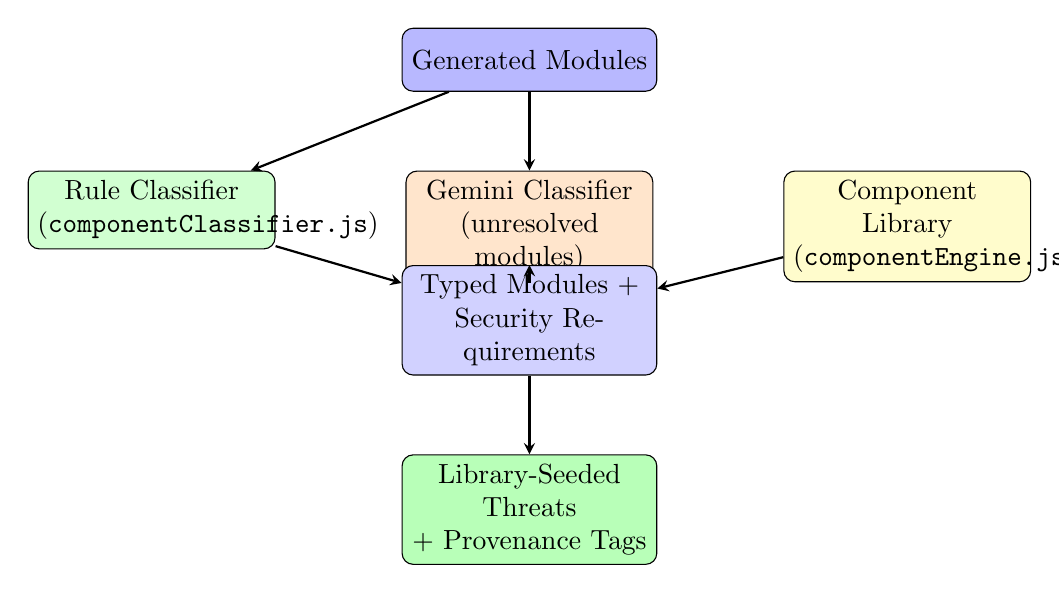
\begin{tikzpicture}[
    node distance=1.0cm and 1.6cm,
    box/.style={rectangle, draw, rounded corners, text width=3.0cm, text centered, minimum height=0.8cm, fill=blue!18},
    proc/.style={rectangle, draw, rounded corners, text width=2.9cm, text centered, minimum height=0.8cm, fill=green!18},
    data/.style={rectangle, draw, rounded corners, text width=2.9cm, text centered, minimum height=0.8cm, fill=yellow!20},
    ext/.style={rectangle, draw, rounded corners, text width=2.9cm, text centered, minimum height=0.8cm, fill=orange!20},
    arrow/.style={->, >=stealth, thick}
]
    \node[box, fill=blue!28] (mods) {Generated Modules};
    \node[proc, below left=of mods] (rules) {Rule Classifier\\(\texttt{componentClassifier.js})};
    \node[ext, below=of mods] (ai) {Gemini Classifier\\(unresolved modules)};
    \node[data, below right=of mods] (lib) {Component Library\\(\texttt{componentEngine.js})};
    \node[box, below=2.2cm of mods] (typed) {Typed Modules +\\Security Requirements};
    \node[box, below=of typed, fill=green!28] (seed) {Library-Seeded Threats\\+ Provenance Tags};

    \draw[arrow] (mods) -- (rules);
    \draw[arrow] (mods) -- (ai);
    \draw[arrow] (rules) -- (typed);
    \draw[arrow] (ai) -- (typed);
    \draw[arrow] (lib) -- (typed);
    \draw[arrow] (typed) -- (seed);
\end{tikzpicture}

\section{DFD and Trust-Boundary Analysis}
The tool supports two modeling paths:
\begin{enumerate}
    \item \textbf{Auto DFD mode}: generates Level-0 and Level-1 SVG diagrams directly from modules and flows.
    \item \textbf{Interactive canvas mode}: analysts draw entities/processes/stores/boundaries manually in a visual editor.
\end{enumerate}

Trust boundaries can be manually assigned per module, and Gemini can produce supplementary high-risk flow notes.

\begin{tikzpicture}[
    node distance=1.1cm and 1.8cm,
    mode/.style={rectangle, draw, rounded corners, text width=3.1cm, text centered, minimum height=0.85cm, fill=blue!17},
    proc/.style={rectangle, draw, rounded corners, text width=3cm, text centered, minimum height=0.85cm, fill=green!17},
    out/.style={rectangle, draw, rounded corners, text width=3.2cm, text centered, minimum height=0.9cm, fill=yellow!20},
    arrow/.style={->, >=stealth, thick}
]
    \node[mode, fill=blue!25] (auto) {Auto DFD Mode\\(Context + Level-1)};
    \node[mode, right=of auto, fill=blue!25] (canvas) {Interactive Canvas\\(\texttt{ThreatModelerCanvas.jsx})};
    \node[proc, below=of auto] (tb) {Manual Trust Boundary\\Annotations};
    \node[proc, below=of canvas] (aian) {Gemini Boundary/Flow\\Risk Analysis};
    \node[out, below=1.8cm of $(tb)!0.5!(aian)$] (out) {Cross-Boundary Flow Set\\+ Security Notes for STRIDE};

    \draw[arrow] (auto) -- (tb);
    \draw[arrow] (canvas) -- (tb);
    \draw[arrow] (canvas) -- (aian);
    \draw[arrow] (tb) -- (out);
    \draw[arrow] (aian) -- (out);
\end{tikzpicture}

\newpage
\section{Threat Lifecycle: STRIDE to DREAD to Report}
\begin{tikzpicture}[
    node distance=1.05cm and 1.6cm,
    proc/.style={rectangle, draw, rounded corners, text width=3.2cm, text centered, minimum height=0.85cm, fill=green!18},
    data/.style={rectangle, draw, rounded corners, text width=2.9cm, text centered, minimum height=0.78cm, fill=yellow!22},
    out/.style={rectangle, draw, rounded corners, text width=3.2cm, text centered, minimum height=0.9cm, fill=blue!20},
    arrow/.style={->, >=stealth, thick}
]
    \node[proc, fill=green!25] (seed) {Threat Inputs\\(library + questionnaire + AI + manual)};
    \node[data, below left=of seed] (stride) {STRIDE Category\\Normalization};
    \node[data, below=of seed] (status) {Analyst Triage\\(applicable/review/NA)};
    \node[data, below right=of seed] (dread) {DREAD Scoring\\(5 dimensions)};
    \node[out, below=2.0cm of seed] (ranked) {Ranked Threat Register\\(critical/high/medium/low)};
    \node[out, below=of ranked, fill=blue!28] (report) {Executive Report\\+ Mitigations + JSON Export};

    \draw[arrow] (seed) -- (stride);
    \draw[arrow] (seed) -- (status);
    \draw[arrow] (seed) -- (dread);
    \draw[arrow] (stride) -- (ranked);
    \draw[arrow] (status) -- (ranked);
    \draw[arrow] (dread) -- (ranked);
    \draw[arrow] (ranked) -- (report);
\end{tikzpicture}

\section{Core Data Model}
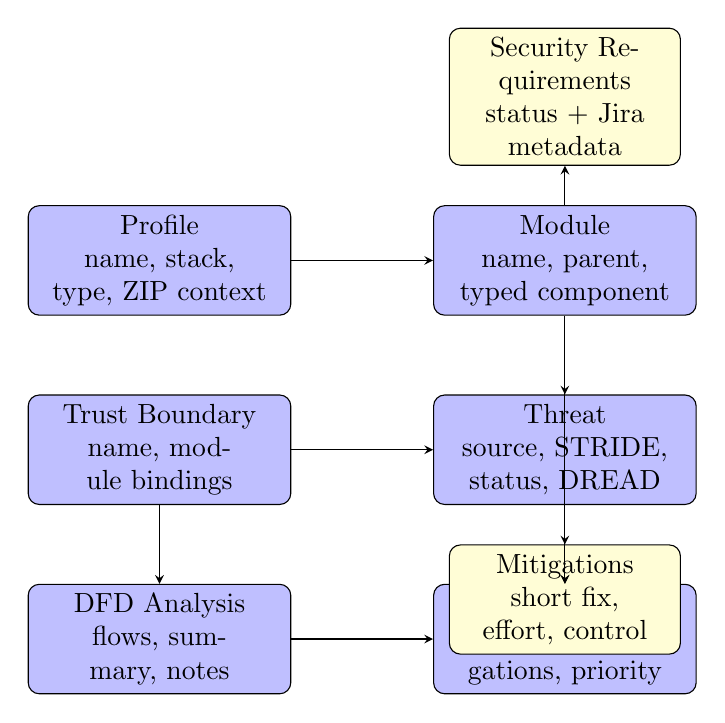
\begin{tikzpicture}[
    node distance=1cm and 1.8cm,
    entity/.style={rectangle, draw, rounded corners, text width=3.1cm, text centered, minimum height=0.95cm, fill=blue!15},
    field/.style={rectangle, draw, rounded corners, text width=2.7cm, text centered, minimum height=0.7cm, fill=yellow!16},
    arrow/.style={->, >=stealth}
]
    \node[entity, fill=blue!25] (profile) {Profile\\name, stack, type, ZIP context};
    \node[entity, right=of profile, fill=blue!25] (module) {Module\\name, parent, typed component};
    \node[entity, below=of module, fill=blue!25] (threat) {Threat\\source, STRIDE, status, DREAD};
    \node[entity, left=of threat, fill=blue!25] (boundary) {Trust Boundary\\name, module bindings};
    \node[entity, below=of boundary, fill=blue!25] (dfd) {DFD Analysis\\flows, summary, notes};
    \node[entity, right=of dfd, fill=blue!25] (report) {Report Payload\\bySource, mitigations, priority};

    \node[field, above=0.5cm of module] (req) {Security Requirements\\status + Jira metadata};
    \node[field, below=0.5cm of threat] (mit) {Mitigations\\short fix, effort, control};

    \draw[arrow] (profile) -- (module);
    \draw[arrow] (module) -- (threat);
    \draw[arrow] (module) -- (req);
    \draw[arrow] (boundary) -- (threat);
    \draw[arrow] (boundary) -- (dfd);
    \draw[arrow] (threat) -- (mit);
    \draw[arrow] (threat) -- (report);
    \draw[arrow] (dfd) -- (report);
    \draw[arrow] (module) -- (report);
\end{tikzpicture}

\newpage
\section{Experimental Utility and Demonstration Corpus}
The repository includes two benchmark-style demo projects under \texttt{testing/}:
\begin{itemize}
    \item \texttt{legacy-hr-portal}: legacy monolith patterns yielding dense code-level STRIDE findings.
    \item \texttt{modern-notes-saas}: modern service architecture yielding boundary and integration-centric threats.
\end{itemize}

This paired corpus is useful for evaluating model sensitivity across two regimes:
\begin{enumerate}
    \item explicit insecure coding patterns in legacy systems;
    \item emergent trust and lifecycle threats in modern distributed SaaS systems.
\end{enumerate}

\section{Security and Design Properties}
\begin{itemize}
    \item \textbf{Grounded inference}: deterministic signals constrain generative hallucination.
    \item \textbf{Provenance-aware threats}: source tags distinguish library, questionnaire, AI, and manual findings.
    \item \textbf{Analyst override-first}: all outputs remain editable before reporting.
    \item \textbf{Browser-local preprocessing}: ZIP extraction and module derivation run client-side.
    \item \textbf{Governance readiness}: structured report payload includes requirement status and test-frequency recommendation.
\end{itemize}

\section{Limitations and Future Directions}
\begin{itemize}
    \item LLM quality is bounded by context quality and API availability.
    \item Import-graph extraction currently targets JS/TS ecosystems most strongly.
    \item Risk scoring remains expert-judgment-driven and can vary across analysts.
\end{itemize}

Future work can extend multi-language static extraction, differential threat-model versioning, and automated validation of mitigation closure against CI artifacts.

\section{Conclusion}
Lightweight Threat Modeler operationalizes a practical hybrid architecture for modern threat modeling: deterministic repository intelligence, taxonomy-driven security knowledge, and selective AI augmentation. The result is an interpretable, iterative, and exportable STRIDE/DREAD workflow suited for both architecture design reviews and implementation-oriented security engineering.

\end{document}
